\documentclass[a4paper,12pt,twoside]{article}

\usepackage[utf8]{inputenc}
\usepackage[pdftex]{graphicx}
\usepackage[pdftex]{hyperref}
\usepackage{float}
\usepackage[margin=3cm]{geometry}
\usepackage[english]{babel}
\usepackage{subcaption}

\begin{document}
  
\section {The Temperature of a Given Day}

The aim of this part of the project is to find the temperature of a given day of the year. The day chosen for this analysis is March 3rd. For the sake of comparison two datasets are chosen: Luleå (located in the north of Sweden) and Lund (located in the south). \\

\noindent In order to analyze the data, a function called ``tempOnday" was defined. Inside the function, which accepted two arguments: the month and the day to be analyzed, a for loop which ran through all the data points - except the last one - was created. Inside the for loop the code first controlled if the data point corresponded to the month and the day given as 
arguments to the function. If it did, the temperature corresponding to this data point was added to a variable called ``tempYear". The amount of times this was done was tracked with a counter. The code continued with controlling if the year of the current data point was the same as the consecutive year. If this
was not the case, and the current year differed from the consecutive one, the variable ``tempYear" was divided by the counter (that is, by the amount of times a new temperature had been added to the variable). This was done because in the dataset several temperatures were given for each day, and thus this way 
the average temperature for March third on each year was calculated. When this average was calculated, it was saved inside a vector ``tempVec" for later use and the counter and variable ``tempYear" were reseted. In a final if-statement it was checked if the data point was the last one. This because the original for 
loop, only looped through until the second last data point. Thus if the current data point was the last, the variable ``tempYear" was also divided by the counter and an average for the last year in the dataset was obtained and saved in the vector ``tempVec". 
When the for loop was finished the vectors obtained (one for each city) were used to fill the histograms shown in figure \ref{fig:histos}. After the histograms were made, the mean temperature of the given day together with the standard deviation of the temperatures were found through the histograms, but also by calculation. \\

\begin{figure}[H]
\centering
\begin{subfigure}{.5\textwidth}
  \centering
  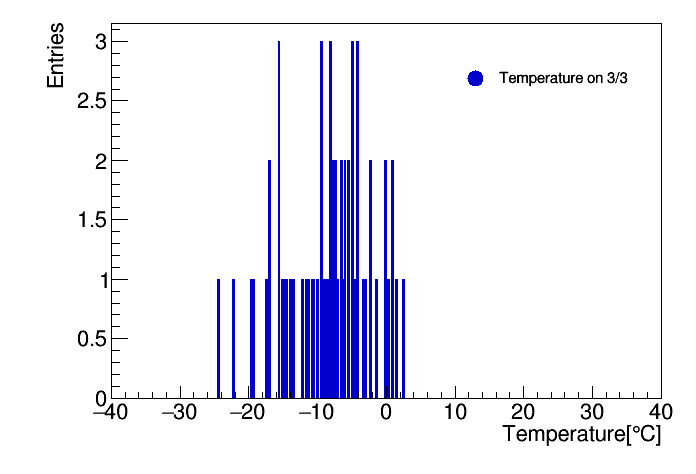
\includegraphics[width=1.0\linewidth]{Lulea.png}
  \caption{Luleå dataset.}
  \label{fig:Lulea}
\end{subfigure}%
\begin{subfigure}{.5\textwidth}
  \centering
  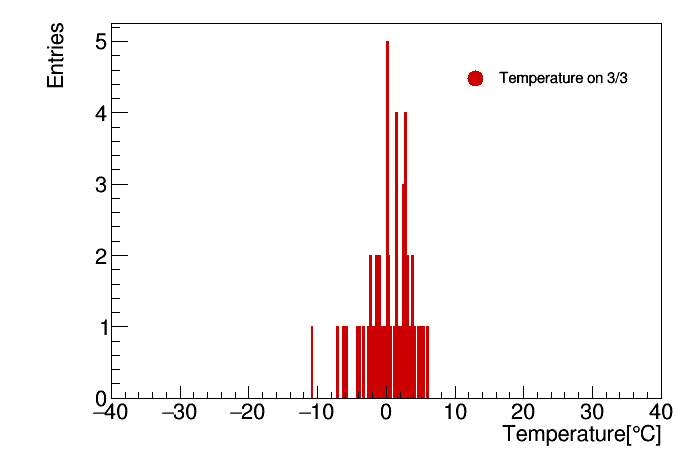
\includegraphics[width=1.0\linewidth]{Lund.png}
  \caption{Lund dataset.}
  \label{fig:Lund}
\end{subfigure}
\caption{The temperature of March 3rd.}
\label{fig:histos}
\end{figure}

\noindent In figure \ref{fig:Lulea} and \ref{fig:Lund} the histograms created with the Luleå and Lund datasets respectively, can be seen. The mean temperature in Luleå on March third according to the histogram (and the calculations) is $-8.37 \pm 6.02 ^\circ$ C. While in Lund the mean temperature on the same day is $0.44 \pm 3.33 ^\circ$ C. As can be seen the mean 
temperature in Lund is much higher than the one in Luleå, which is not strange considering the locations of these two cities. Another thing to notice is the difference in the standard deviations, which is smaller for the Lund dataset than for the Luleå dataset. This can also be directly seen from the histograms in figure \ref{fig:histos}. 

\end{document}
